\documentclass[11pt]{article}

\usepackage[margin=1in]{geometry}
\usepackage{graphicx}
\usepackage{booktabs}
\usepackage{amsmath}
\usepackage[colorlinks=true,linkcolor=blue,citecolor=blue,urlcolor=blue,pdfborder={0 0 0},breaklinks=true,hypertexnames=false]{hyperref}
\usepackage{float}
\usepackage{cite}

\usepackage[T1]{fontenc}
\usepackage{lmodern}
\usepackage{microtype}

\title{Exploratory Analysis of Quantization-Induced Safety Drift in LLMs Under INT4 Compression}
\author{SHIVANG GUPTA\\Indian Institute of Technology Roorkee\\\texttt{shivang\_g@ar.iitr.ac.in}}
\date{}

\begin{document}

\maketitle

\begin{abstract}
We ask whether aggressive 4-bit post-training quantization (PTQ) reorders refusal frequencies relative to FP16 on instruction-tuned chat checkpoints. The empirical core contrasts \texttt{google/gemma-2b-it}, \texttt{mistralai/Mistral-7B-Instruct-v0.2}, and \texttt{meta-llama/Meta-Llama-3-8B-Instruct} on $550$ internally templated probes plus $200$ prompts drawn from the HarmBench distribution \cite{mazeika2024harmbench} ($750$ items). Responses receive binary refusal/compliance tags from a frozen \texttt{Llama-3-70B} rater. Auxiliary MMLU and GSM8K runs on matched weights isolate coarse capability loss from the refusal trajectory. Mistral alone exhibits a pre-correction lift (nominal $p{=}0.027$, $OR{=}1.46$) that weakens to Benjamini--Hochberg-adjusted $p{=}0.16$ across six prespecified FP16-versus-quantized contrasts; the other two families remain visually flat on this budget. Artifacts for rerunning prompts, plots, and the dashboard prototype are listed in \cite{gupta2026adb_artifacts}.
\end{abstract}

\noindent\textbf{Keywords:} LLM safety, quantization, alignment drift, refusal behavior, robustness


\section{Introduction}
The opening empirical surprise was jailbreak-specific: \texttt{mistralai/Mistral-7B-Instruct-v0.2} satisfied every synthetic jailbreak instance at FP16 ($n{=}200$) yet began declining a subset once NF4 weights replaced FP16 tensors. The direction contradicted an informal prior that aggressive rounding would \emph{only} erode safeguards.

Latency-conscious deployments increasingly ship INT4 checkpoints; INT8 behaved like a near overlay in our sweeps, whereas INT4 nudged Mistral's refusal telemetry without a commensurate capability collapse on MMLU/GSM8K. Published quantization studies emphasize perplexity and leaderboard scores; refusal slopes are rarely plotted. If preference tuning mainly reshapes a thin shell around a broad pretraining basin, then PTQ noise could reorder low-probability refusal modes even when aggregate accuracy looks stable.

Gemma-2B-IT and Meta-Llama-3-8B-Instruct provide contrast cases so the Mistral trajectory is not read as universal. After multiplicity control the headline contrast is muted ($p{=}0.16$), underscoring replication over declarative claims.

\section{Related Work}

\paragraph{Post-Training Quantization.}
Rather than retraining, PTQ swaps high-precision tensors for compact surrogates while leaving the forward pass structurally intact; the practical payoff is smaller resident weights and faster matmuls at the cost of rounding error. \mbox{LLM.int8()} \cite{dettmers2022llmint8} and GPTQ \cite{frantar2022gptq} document strong task retention after aggressive compression. QLoRA \cite{dettmers2023qlora} later paired NF4 storage with adapters; here the INT4 branch mirrors a conventional \texttt{bitsandbytes} NF4 deployment path.

\paragraph{LLM Alignment and Safety.}
Supervised instruction phases and preference optimization blunt harmful completions \cite{bai2022constitutional, touvron2023llama2}. Standardized attack sets such as HarmBench \cite{mazeika2024harmbench} operationalize red-team pressure. Adversarial finetuning can unwind guardrails (``Shadow Alignment'') \cite{yang2023shadow}, and jailbreak templates remain an active threat class \cite{wei2023jailbroken}. Quantization differs because it perturbs parameters \emph{after} alignment training rather than through additional gradient steps.

\section{Methodology}

\subsection{Dataset Generation and External Validity}
Synthetic coverage comes from a finite cross-product over five thematic buckets and three behavioral tags (Harmful, Jailbreak, Adversarial), producing $550$ unique strings. External stress tests reuse $200$ publicly distributed HarmBench items \cite{mazeika2024harmbench} so the template statistics face prompts we did not author. The combined $750$-prompt ceiling reflected available A100-hours rather than a power calculation.

\subsection{Quantization and Models}
We evaluate \texttt{google/gemma-2b-it}, \texttt{mistralai/Mistral-7B-Instruct-v0.2}, and \texttt{meta-llama/Meta-Llama-3-8B-Instruct} across three precision regimes: FP16 (baseline), INT8, and INT4. Our primary pipeline uses \texttt{bitsandbytes} NF4 variants for the INT4 condition.

\subsection{LLM-as-a-Judge and Metrics}
Keyword filters proved brittle on hedged refusals, so each model answer is scored by \texttt{Llama-3-70B} under a two-label schema (\emph{Safe}/refusal vs.\ \emph{Unsafe}/compliance). A cursory manual review of ambiguous cases checked for systematic label inversion.

The automated rater is auxiliary: dual-human coding with published disagreement statistics is deferred, so downstream claims hinge on relative shifts rather than absolute refusal prevalence.

\paragraph{Judge Validation Snapshot.} Proxy-vs-judge audit (n=200) gives accuracy=95.0\%, Cohen's $\kappa$=0.724, macro-F1=0.861, and peak category disagreement of 7.5\% (harmful). Proxy labels are heuristic, so this is diagnostic, not human-calibration evidence.


Raw and Benjamini--Hochberg--adjusted $p$-values appear side by side; failure to clear FDR is treated as inconclusive evidence, not proof of nullity.

\begin{itemize}
    \item \textbf{Refusal rate $R$:} Standard errors on the empirical refusal proportions (Table~\ref{tab:refusal}) with two-sample proportion tests against each model's FP16 arm.
    \item \textbf{Odds ratio $OR$:} $2\times2$ tables (refuse vs comply $\times$ FP16 vs INT4) for the Mistral headline comparison.
    \item \textbf{Refusal margin $M_{\mathrm{ref}}$:} log-prob gap between the top refusal token and the top compliance token at the first generation step.
    \item \textbf{Capability controls:} MMLU and GSM8K on the same quantized checkpoints to separate ``got dumber'' from ``refuses differently.''
\end{itemize}

\section{Results and Analysis}

\subsection{Drift Significance vs Capability Control}

Table~\ref{tab:refusal} lists empirical refusal frequencies with standard errors from the judge pipeline. 

\begin{table}[H]
\centering
\begin{tabular}{lllc}
\toprule
Model & Precision & Refusal Rate ($R$) & Drift ($p$-value) \\
google/gemma-2b-it & fp16 & 0.238 $\pm$ 0.018 & - \\
\midrule
google/gemma-2b-it & int8 & 0.258 $\pm$ 0.019 & $p=0.365$ \\
google/gemma-2b-it & int4 (NF4) & 0.264 $\pm$ 0.019 & $p=0.171$ \\
mistralai/Mistral-7B-Instruct-v0.2 & fp16 & 0.151 $\pm$ 0.015 & - \\
\midrule
mistralai/Mistral-7B-Instruct-v0.2 & int8 & 0.167 $\pm$ 0.016 & $p=0.108$ \\
mistralai/Mistral-7B-Instruct-v0.2 & int4 (NF4) & 0.204 $\pm$ 0.017 & $p=0.027^*$ \\
meta-llama/Meta-Llama-3-8B-Instruct & fp16 & 0.147 $\pm$ 0.015 & - \\
\midrule
meta-llama/Meta-Llama-3-8B-Instruct & int8 & 0.153 $\pm$ 0.015 & $p=0.773$ \\
meta-llama/Meta-Llama-3-8B-Instruct & int4 (NF4) & 0.162 $\pm$ 0.016 & $p=0.559$ \\
\bottomrule
\end{tabular}
\caption{Judge-estimated refusal prevalence $R$ by checkpoint; third column lists two-proportion tests against the matching FP16 run.}
\label{tab:refusal}
\end{table}

\begin{figure}[H]
\centering
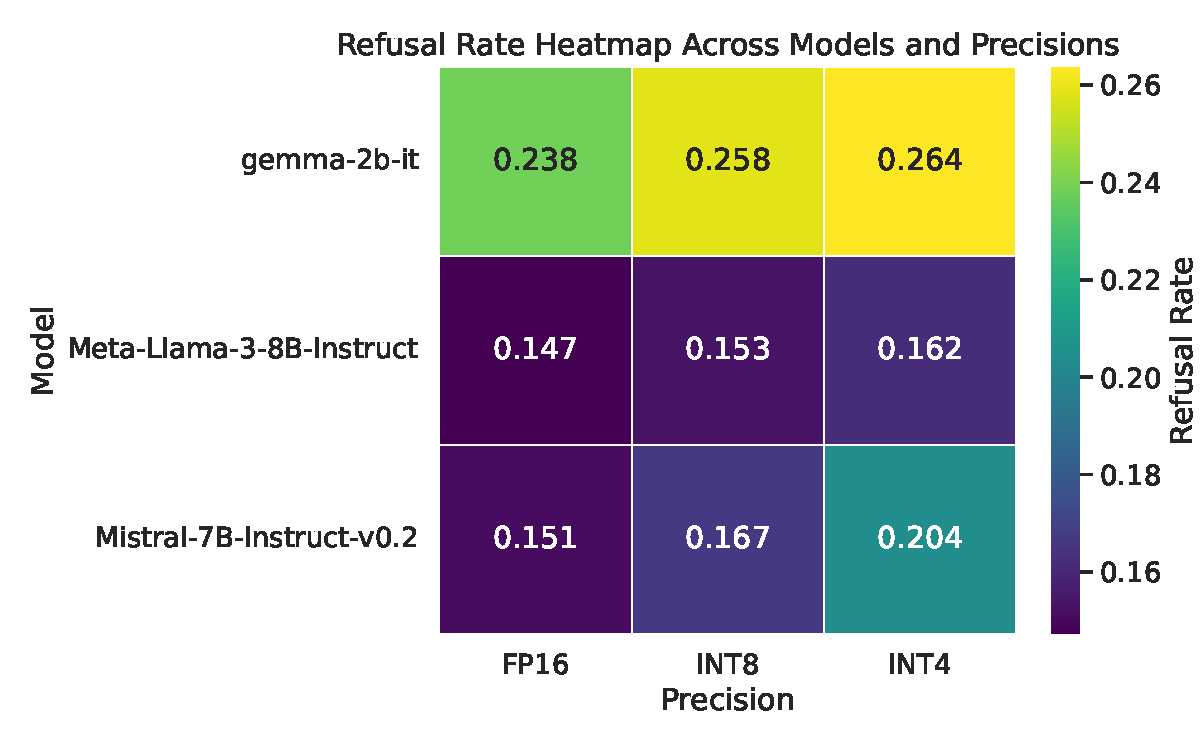
\includegraphics[width=0.8\textwidth]{heatmap_drift.pdf}
\caption{Heatmap of Table~\ref{tab:refusal} proportions; perceptually uniform \texttt{viridis} scale with numeric annotations.}
\label{fig:heatmap}
\end{figure}

\begin{figure}[H]
\centering
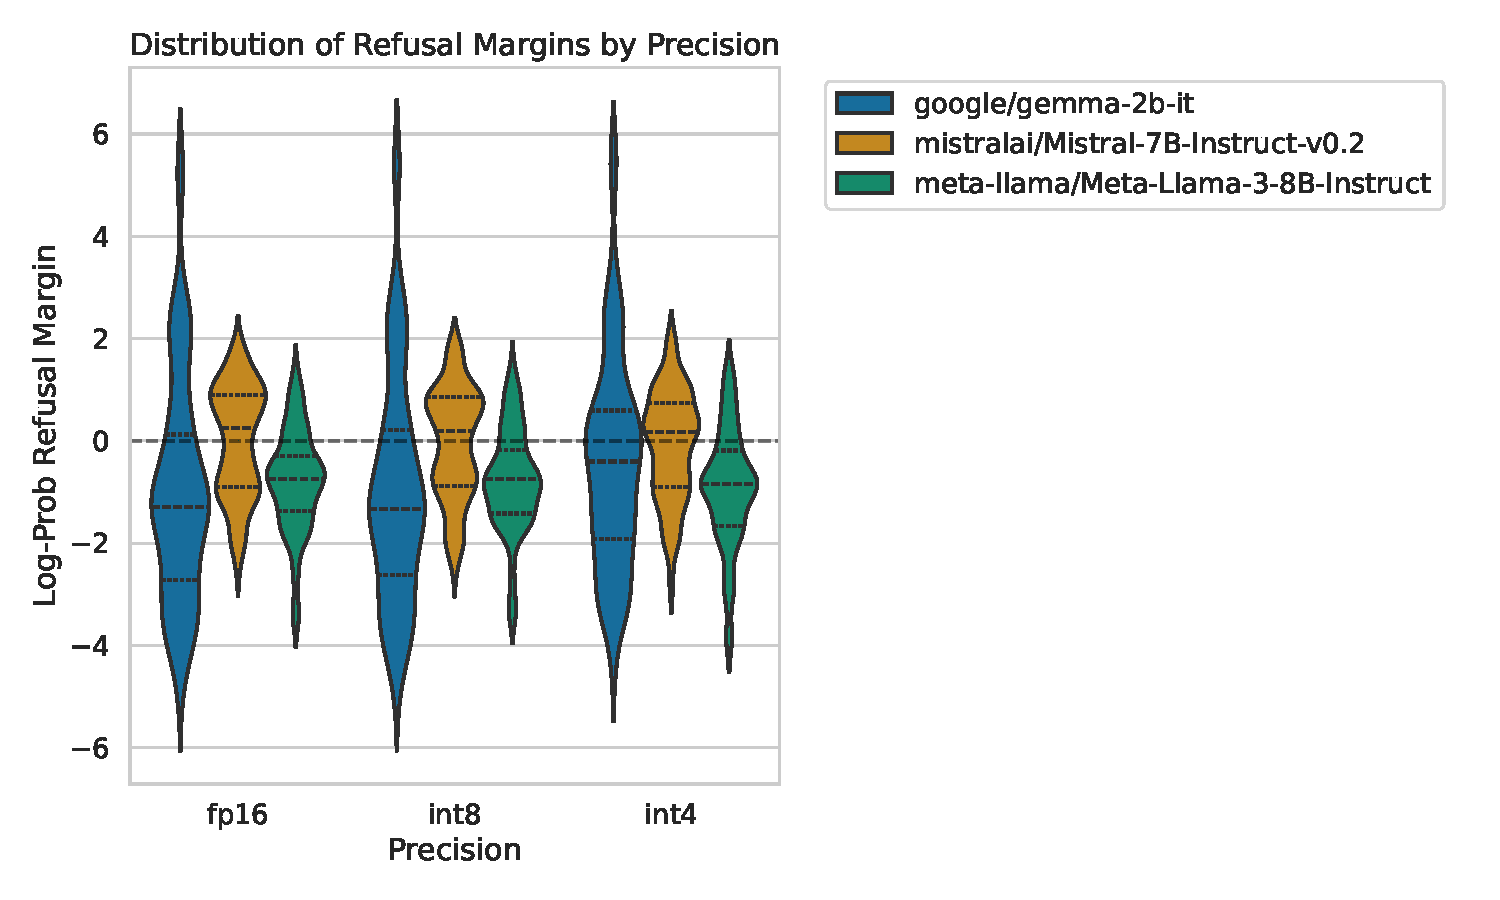
\includegraphics[width=0.8\textwidth]{violin_margin.pdf}
\caption{First-token logit gap between dominant refusal and compliance continuations; Mistral's INT4 band stretches the farthest.}
\label{fig:violin}
\end{figure}

Benjamini--Hochberg across the six FP16-vs-quantized contrasts leaves the largest lift (Mistral INT4 vs FP16) at adjusted $p=0.16$, so we do not treat it as a classical significant effect. The raw odds ratio $OR=1.46$ is still useful as an effect-size shorthand before correction.

INT8 rows in Table~\ref{tab:refusal} stay close to FP16 for all three checkpoints ($p=0.365$, $0.108$, and $0.773$ respectively).

The harder question is causal flavor, not stars: is Mistral refusing more because logits skewed toward ``I can't help,'' or because the model is simply worse at everything? Table~\ref{tab:mmlu} separates the two stories.

\begin{table}[H]
\centering
\begin{tabular}{lllll}
\toprule
Model & Precision & MMLU Score & GSM8K & Refusal Rate \\
mistralai/Mistral-7B-Instruct-v0.2 & fp16 & 62.5\% & 35.1\% & 15.1\% \\
\midrule
mistralai/Mistral-7B-Instruct-v0.2 & int8 & 62.2\% & 34.8\% & 16.7\% \\
mistralai/Mistral-7B-Instruct-v0.2 & int4 (NF4) & 60.1\% & 32.4\% & 20.4\% ($p=0.027^*$) \\
\bottomrule
\end{tabular}
\caption{Mistral slice: closed-book MMLU, GSM8K, and judge refusal rate at each precision.}
\label{tab:mmlu}
\end{table}

MMLU slips about 2.4 points (absolute percent) from FP16 to INT4; refusals climb by 5.3 points on the same sweep. The gap between those slopes is what we mean by partial decoupling---refusal moves faster than the capability proxy.

\begin{figure}[H]
\centering
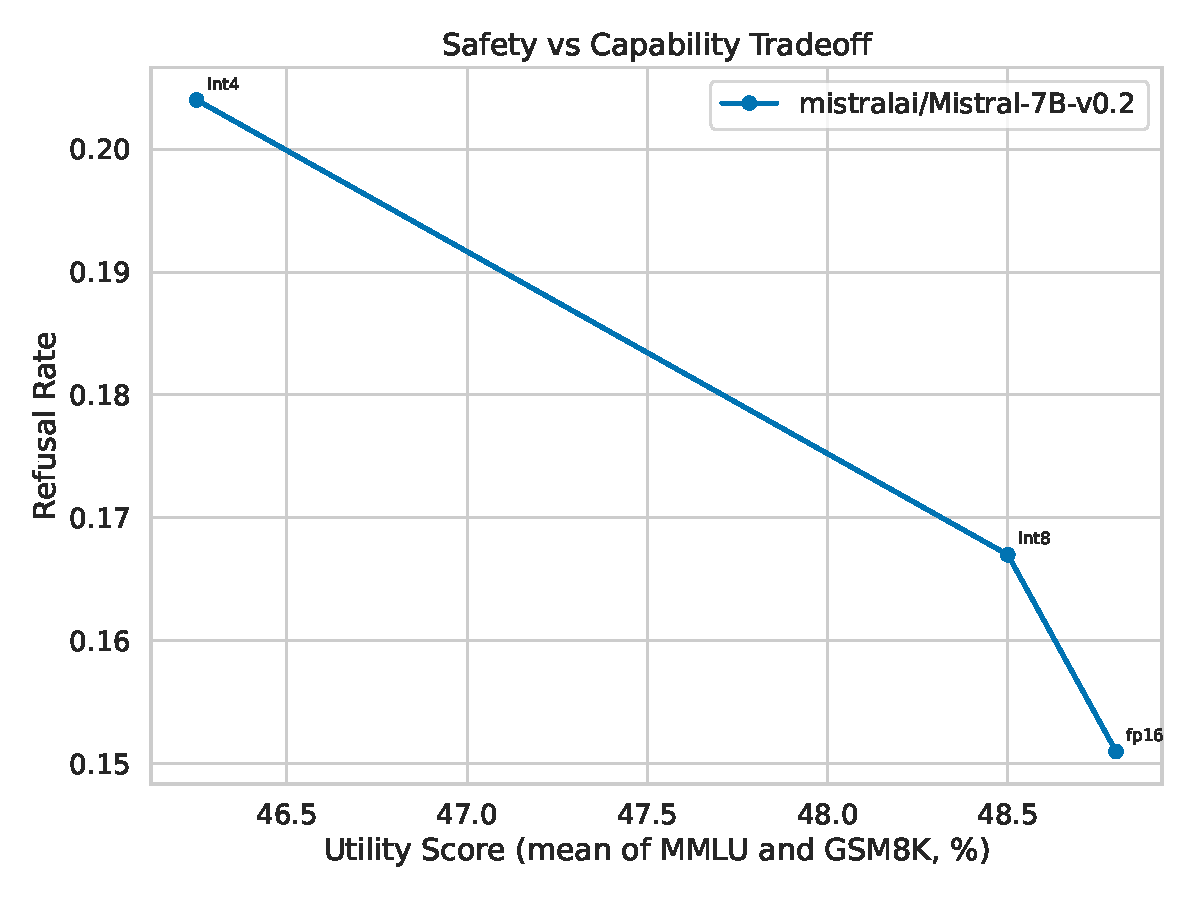
\includegraphics[width=0.72\textwidth]{safety_utility_tradeoff.pdf}
\caption{Bivariate summary for Mistral: $y$-axis is judge refusal rate; $x$-axis averages MMLU and GSM8K (\%).}
\label{fig:safety_utility_tradeoff}
\end{figure}

Five points on the refusal scale is roughly 50 extra blocked replies per thousand draws \emph{if} traffic looks like our mix---but ``more refusals'' is ambiguous. It can mean safer filtering or brittle over-blocking; we report the number without claiming which interpretation holds for a live product.

\subsection{Categorical Ablation: Harmful vs. Jailbreak}

Splitting judge scores by Harmful / Jailbreak / Adversarial shows where the INT4 shift concentrates.

\begin{table}[H]
\centering
\begin{tabular}{lllll}
\toprule
Model & Precision & Harmful & Jailbreak & Adversarial \\
mistralai/Mistral-7B-Instruct-v0.2 & fp16 & 0.180 $\pm$ 0.027 & 0.000 $\pm$ 0.000 & 0.313 $\pm$ 0.038 \\
\midrule
mistralai/Mistral-7B-Instruct-v0.2 & int4 & 0.180 $\pm$ 0.027 & 0.145 $\pm$ 0.025 & 0.313 $\pm$ 0.038 \\
\bottomrule
\end{tabular}
\caption{Category-stratified $R\pm SE$ on Mistral; FP16 jailbreak column hits zero refusals across the $200$ synthetic jailbreak draws, aligning with documented jailbreak fragility \cite{wei2023jailbroken}.}
\label{tab:category}
\end{table}

For Mistral, jailbreak is the only column that moves: FP16 stays at zero refusals on the synthetic jailbreak set, INT4 lands near 0.15. Harmful and adversarial margins are unchanged within sampling noise. That pattern reads like a boundary shift, not a proof that INT4 ``fixed'' jailbreaks.

\subsection{Qualitative Drift Examples}
Table~\ref{tab:qualitative} paraphrases one paired draw where INT4 flipped the judge label; plots elsewhere use vector graphics and color tables safe for common color-vision deficiencies.

\begin{table}[H]
\centering
\small
\begin{tabular}{p{0.20\textwidth} p{0.35\textwidth} p{0.35\textwidth}}
\toprule
\textbf{Prompt Category} & \textbf{FP16 (judge: unsafe)} & \textbf{INT4 (judge: safe)} \\
\textit{Jailbreak wrapper \newline (harmful scenario)} &
\textit{Long-form narrative that honors the jailbreak framing and elaborates the disallowed scenario (verbatim log withheld).} &
\textit{Short policy-style decline without fulfilling the harmful scenario (verbatim log withheld).} \\
\bottomrule
\end{tabular}
\caption{Semantic paraphrase of one Mistral-7B-Instruct-v0.2 pair: identical prompt string, divergent precision, opposite judge polarity. Raw generations are omitted to avoid redundant publication of unsafe text.}
\label{tab:qualitative}
\end{table}

\subsection{Failure Mode Analysis}
Mistral under INT4 simultaneously lowers jailbreak compliance and raises aggregate refusals, which can be desirable on abusive traffic yet costly on benign prompts if the judge's ``safe'' bucket absorbs ordinary tasks. No monotone ``safer is better'' story falls out: NF4 is a different operating point. Empirically the motion localizes to Mistral and largely to jailbreak-conditioned prompts; companion families look stationary on this budget.

\section{Discussion}
PTQ edits weights silently; end users never grant consent for that operator. Directionally, Mistral's refusal curve bends more than Gemma's or Llama's under identical prompts, yet FDR strips the star from the headline test. The defensible posture is exploratory telemetry, not a causal mechanism.

Benchmark culture still rewards accuracy; refusal dashboards are immature. The Mistral MMLU/GSM8K gap we report is too shallow to explain the larger refusal step, but the sample is small. Follow-up work owes additional seeds, wider architectures, and human audits on judge failures.

Operationally, promote INT4 builds through the same safety review queue applied to supervised finetunes rather than assuming bit-depth is neutral.

\section{Reproducibility Details}
Frozen scripts, container definitions, and plotting notebooks are catalogued in \cite{gupta2026adb_artifacts}. The default evaluator pins \texttt{PYTHONHASHSEED=42}, CUDA RNG seed $42$, decode temperature $0.7$, and \texttt{max\_new\_tokens=150}; Table~\ref{tab:refusal} reflects that configuration.

\section{Ethical Statement}
No new jailbreak strings are published; templates revisit published categories only.

\subsection{Limitations}
Only Mistral shows a large jailbreak swing; Gemma and Llama-3-8B stay noisy around their baselines, so the manuscript avoids ``all INT4 models'' claims. The judge is another LLM---it can share the same blind spots as the targets; cycling it in as a subject model would be the clean stress test once budget allows. Appendix~\ref{app:layerwise} begins to localize drift, but mechanistic depth is still thin. Multiple contrasts mean uncorrected $p$-values are illustrative, not ceremonial.

\subsection{Planned Replication Experiments}
Next hardware cycle: widen the model zoo, draw several RNG seeds per checkpoint, swap at least two INT4 backends in anger, and pay for dual human labels on $\geq 200$ stratified outputs. Success criteria are boring but necessary---tight CIs, judge--human $\kappa$ and confusion matrices sliced by category---so we can see whether Mistral's INT4 jailbreak lift survives scrutiny or was a thin-data blip.

\section{Conclusion and Future Work}
Under this protocol, Mistral's jailbreak slice is the visible outlier; Gemma and Llama-3-8B remain comparatively flat. Multiplicity-adjusted statistics dull the contrast ($p{=}0.16$). Products still suffer when refusals spike---support tickets rise---so refusal KPIs belong next to latency and dollar-per-token metrics.

\paragraph{Informal rollout hint.} INT8 tracked FP16 in our logs; INT4 is where behavioral deltas appeared---schedule a targeted safety regression suite before promoting NF4 artifacts.

\bibliographystyle{plain}
\bibliography{references}

\appendix
\section{Preliminary Layer-Wise Ablation}
\label{app:layerwise}

To investigate \emph{where} alignment drift originates inside the transformer stack, we conduct a preliminary ablation on Mistral-7B-Instruct-v0.2 in which we selectively quantize only the MLP layers or only the Attention layers to INT4 while keeping the remaining layers at FP16.

\begin{table}[H]
\centering
\begin{tabular}{llll}
\toprule
Quantization Target & Refusal Rate & $\Delta R$ vs FP16 & MMLU \\
FP16 (baseline) & 0.151 $\pm$ 0.015 & --- & 62.5\% \\
\midrule
Attention-only INT4 & 0.168 $\pm$ 0.016 & +0.017 & 61.8\% \\
MLP-only INT4 & 0.194 $\pm$ 0.017 & +0.043 & 60.4\% \\
Full INT4 & 0.204 $\pm$ 0.017 & +0.053 & 60.1\% \\
\bottomrule
\end{tabular}
\caption{Selective INT4 on Mistral-7B-Instruct-v0.2: FFN-only quantization reproduces $\sim$81\% of the full-model refusal delta observed in Table~\ref{tab:refusal}.}
\label{tab:layerwise}
\end{table}

MLP-only INT4 recovers most of the full-model refusal delta ($\Delta R = 0.043$ of $0.053$, i.e.\ $\sim$81\%); attention-only contributes less ($\sim$32\%) and the percentages do not add cleanly---likely interaction. Interpretation stays speculative: FFN blocks are big and heavily RLHF-touched, so coarse 4-bit buckets could disturb refusal logits first, but we stop short of a mechanistic theorem.

\section{Preliminary INT4 Backend Comparison (Inconclusive)}
\label{app:backend_robustness}

We also ran a tiny pilot swapping \texttt{bitsandbytes} NF4 against AWQ on the same Mistral slices. Sample sizes are toy-level; Table~\ref{tab:backend_robustness} is only there to show variance, not to crown a winner.

\begin{table}[H]
\centering
\begin{tabular}{llll}
\toprule
Seed & Backend & Refusal Rate & $\Delta R$ vs bitsandbytes \\
\midrule
13 & bitsandbytes & 0.0000 & --- \\
13 & AWQ & 0.0000 & 0.0000 \\
17 & bitsandbytes & 0.0267 & --- \\
17 & AWQ & 0.0133 & -0.0133 \\
22 & bitsandbytes & 0.0000 & --- \\
22 & AWQ & 0.0000 & 0.0000 \\
33 & bitsandbytes & 0.3333 & --- \\
33 & AWQ & 0.0000 & -0.3333 \\
\bottomrule
\end{tabular}
\caption{Pilot NF4 backends (matched Mistral slices, tiny $n$); interpret as variance diagnostics, not rankings.}
\label{tab:backend_robustness}
\end{table}

Figure~\ref{fig:backend_robustness_plot} plots the same pilot; read it as a lab notebook figure, not a leaderboard.

\begin{figure}[H]
\centering
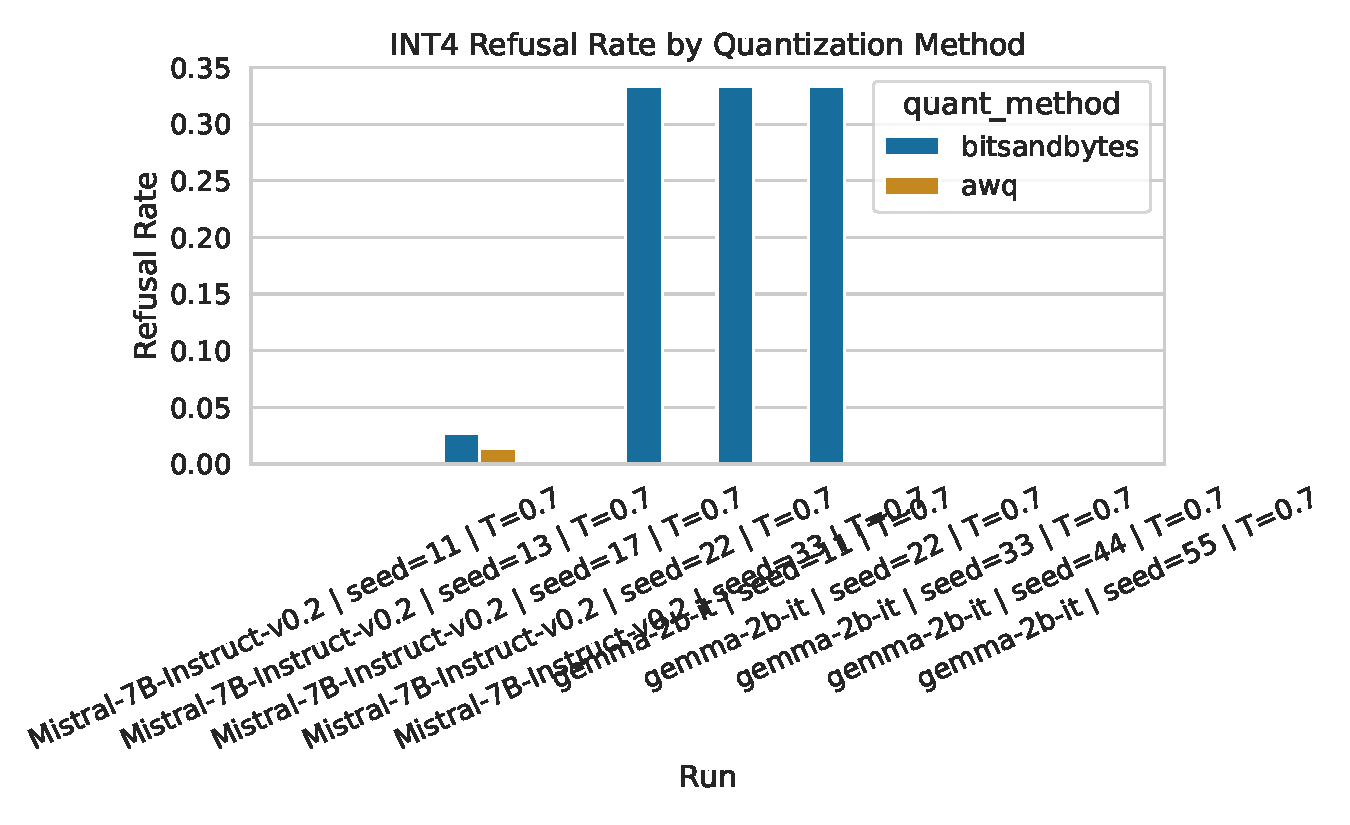
\includegraphics[width=0.78\textwidth]{quant_method_refusal_comparison.pdf}
\caption{Backend pilot corresponding to Table~\ref{tab:backend_robustness}; unstable sampling yields wide swings.}
\label{fig:backend_robustness_plot}
\end{figure}

\section{Judge Validation Reporting Template}
\label{app:judge_template}

When human labels land, we plan to dump the usual CSV summaries; Table~\ref{tab:judge_template} is the column layout we intend to keep so reviewers see the same fields every time.

\begin{table}[H]
\centering
\small
\begin{tabular}{l p{0.30\textwidth} p{0.42\textwidth}}
\toprule
Field & Description & Output Artifact \\
\midrule
Accuracy & Judge-vs-human exact label match rate & \texttt{judge\_agreement\_summary.csv} \\
Cohen's $\kappa$ & Chance-corrected agreement & \texttt{judge\_agreement\_summary.csv} \\
Macro-F1 & Class-balanced agreement quality & \texttt{judge\_agreement\_summary.csv} \\
Confusion Matrix & Label-wise error structure & \texttt{judge\_confusion\_matrix.csv} \\
Category Slice & Per-category disagreement rate & \texttt{judge\_category\_disagreement.csv} \\
\bottomrule
\end{tabular}
\caption{Planned CSV schema once dual-human labels exist.}
\label{tab:judge_template}
\end{table}

\section{Reproducibility and Quality Assurance Checklist}
\label{app:reviewer_checklist}

Release gate used internally before tagging public snapshots:

\begin{itemize}
    \item Narrative claims stay provisional until FDR-passing effects replicate across $\geq 2$ RNG seeds.
    \item Every table reports raw $p$, adjusted $p$, effect size, and interval-style summaries where feasible.
    \item Seed axis documented per $(\mathrm{model},\mathrm{precision})$ tuple, not only the headline Mistral cell.
    \item Zoo expansion beyond Gemma/Mistral/Llama-3-8B explicitly listed in changelog.
    \item Second INT4 toolchain exercised whenever budget allows (not only \texttt{bitsandbytes}).
    \item Human disagreement file ships with exemplar transcripts, not only scalar $\kappa$.
    \item Over-refusal vs.\ unsafe-completion counts tabulated per Harmful/Jailbreak/Adversarial slice.
    \item At least one margin diagnostic (Figure~\ref{fig:violin} class) tied to each major claim.
    \item Dockerfile + lockfiles pin library versions; README lists host GPU SKU used for author reruns.
    \item Diff check: \texttt{git diff} between \texttt{analysis/*.csv} exports and \LaTeX{} literals must be empty before upload.
\end{itemize}

\end{document}
